\documentclass[a4paper,twoside]{article}
\usepackage[hmarginratio=1:1,top=32mm,columnsep=20pt]{geometry} % custom page layout
\usepackage[T1]{fontenc}
\usepackage[utf8]{inputenc}
\usepackage[english]{babel}
\usepackage{lmodern}
\usepackage{fixltx2e} % \textsubscript command
\usepackage{soulutf8} % \ul command
\usepackage{changepage} % indentation (in title page)
\usepackage[font=it]{caption} % captions in italics
\usepackage[font=it]{subcaption} % subcaptions in italics
\usepackage{multicol}
\usepackage{cancel} % \cancel command
\usepackage{textcomp} % symbols
\usepackage{amsmath, amssymb}
\usepackage{amsthm}
\usepackage{makeidx}
\usepackage{graphicx}
\usepackage{float}
\usepackage{wrapfig}


\usepackage{verbatim}
\usepackage{listings}
\lstset{language=vhdl,%
	  keywordstyle=\color{Blue},
      basicstyle=\small\ttfamily,
      frame=TB,
      commentstyle=\color{red},
      showstringspaces=false
}
\usepackage[dvipsnames,usenames]{color}
\usepackage{fancyhdr}

%\usepackage{draftwatermark}
%\SetWatermarkText{Doc interno}



\pagestyle{fancy}
%\renewcommand{\chaptermark}[1]{\markboth{#1}{}}
\renewcommand{\sectionmark}[1]{\markright{ \thesection \space - \space #1}}
\renewcommand{\subsectionmark}[1]{\markright{\thesubsection \space - \space #1}}
\fancyhf{} \fancyhead[RO, LE]{\bfseries \thepage}
 \fancyhead[RE, LO]{
\includegraphics[scale=0.03]{Immagini/262}\bfseries}
\fancyhead[CO, CE]{\bfseries\rightmark}
%\fancyhead[CE]{\bfseries \leftmark}
\renewcommand{\headrulewidth}{0.5pt}
\renewcommand{\footrulewidth}{0pt}
\addtolength{\headheight}{0.5pt} \fancypagestyle{plain}{
\fancyhead{}
\renewcommand{\headrulewidth}{0pt}}

\newtheorem{thm}{Teorema}[section] 
\newtheorem{cor}[thm]{Corollario} 
\newtheorem{lem}[thm]{Lemma} 
\newtheorem{prop}[thm]{Proposizione} 
\theoremstyle{definition} 
\newtheorem{defn}{Definizione}[section]
\theoremstyle{remark} 
\newtheorem{oss}{Osservazione} 
\frenchspacing
\author{Alessandro Salvato}

\newcommand{\paginavuota}{\newpage\null\thispagestyle{empty}\newpage\null}

\begin{document}
\bibliographystyle{unsrt}
\thispagestyle{empty}
\begin{figure}[H]
\centering

\includegraphics[scale=.3]{Immagini/262}
\label{262}
\end{figure}
\begin{center}
\LARGE { \textbf {POLITECNICO DI TORINO} }\\ [1\baselineskip]
%Raccolta di Appunti \\ [2\baselineskip]
\huge{ \textbf{Electronics for Embedded Systems}}\\ [1\baselineskip]
\Huge{\textbf{Project of the course}}\\[1\baselineskip]


\end{center}

\begin{flushleft}
\large{Professor: Claudio Passerone}
\end{flushleft}
\begin{flushleft}
\large{Data: \today}
\end{flushleft}
\begin{flushleft}
\large{Author: Alessandro Salvato} 
\end{flushleft}


\clearpage
\paginavuota

\tableofcontents
\newpage

\section{Introduction}
I'm very glad to present by this report, my own project for Electronics for Embedded Systems course. The main idea consists in  realizing a camera able to capture photos to be transferred to an host computer for further processing. Before describing in details the environmental structure, I guess it's fundamental to highlight that all the topics of the course have been covered in the following manner:
\begin{itemize}
\item \textbf{Memory}: memory controller as FSM
\item \textbf{Programmable logic device}: acts as remote to send the user command
\item \textbf{Interconnection protocol}: I2C, SCCB and UART
\item \textbf{Peripheral management}: programming of camera peripheral
\item \textbf{AD and DA converters}: usage of AD converter to sample the luminance of the environment
\item \textbf{Power management}: Step-down converter to drive a LED
\end{itemize}
Each of them owns a proper section below.
\newline
Let's have a look on the general architecture, listing the main parts of the system. The camera is connected to an ST microcontroller: a STM32F446ZET. The choice on this MCU has due to the fact that it integrates a very useful and widespread engaged peripheral in the video-capturing field: the Digital CaMera Interface (\textbf{DCMI}). All images are sent to the host computer by UART protocol, exploiting another embedded peripheral of the microcontroller. Computer reads UART's data plugging a USB-UART adapter.  Then a small Python script converts those data into a BMP image. 
\newline
The command is generated by the user pushing a specific button. An 8 buttons keyboard is tied up to the FPGA: an Altera Cyclone IV on DE0-Nano board. The implemented VHDL is composed of the keyboard driver and a fully structural UART peripheral. When a button has clicked, an encoded 8-bit data is sent to the microcontroller, which, by an interrupt, recognizes that the user pushed something. 
\newline
A breadboard has been used to build circuits for AD and Bulk converters. For sure, the following image is more clarifying for the reader.
\newline
\newline
I used STM32 CubeIDE to program the microcontroller , a software Eclipse based. To program the FPGA I exploited both Quartus II when uploading the \textit{sof} file and Xilinx ISE Design Suite when simulating (just for my high familiarity with that). Moreover, as classical laboratory instruments I relied on an oscilloscope provided by GW Instek and a multimeter for resistor measurements.
\newline
\newline
Images captured are in the format QVGA
\begin{figure}[H]
\centering
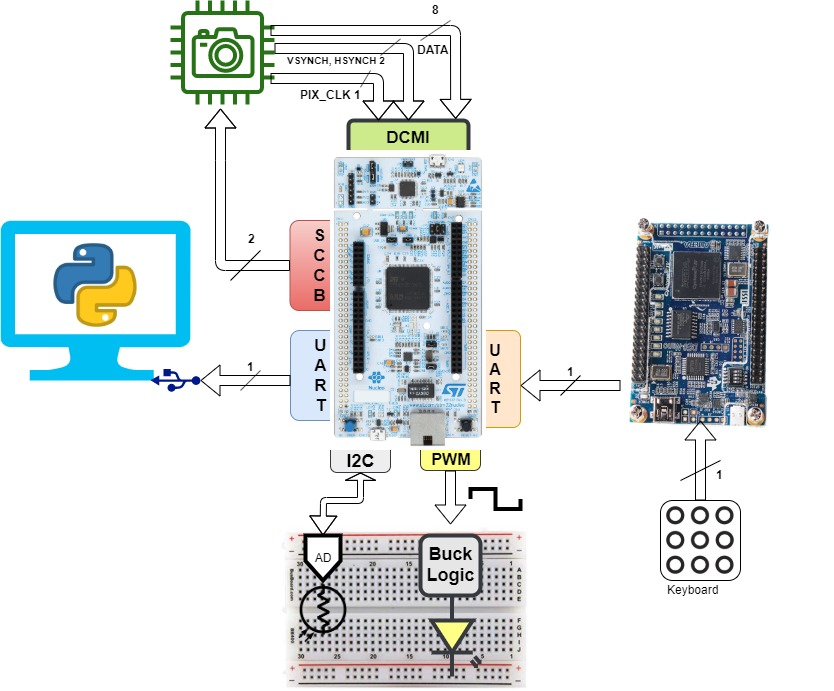
\includegraphics[scale=.5]{Immagini/01}
\label{01}
\caption{General block schema}
\end{figure}

What actually is

\begin{figure}[H]
\centering
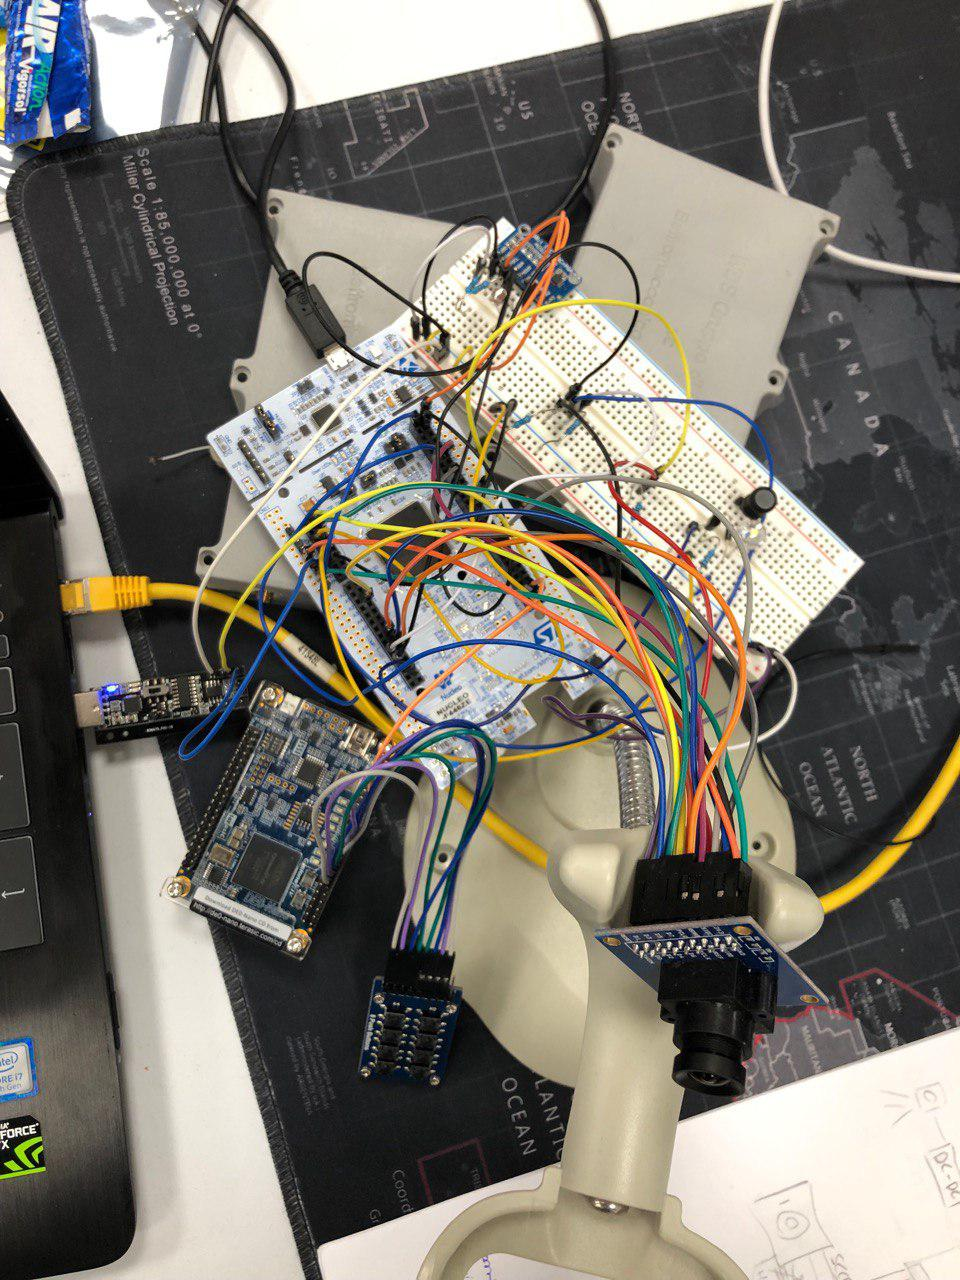
\includegraphics[scale=.4]{Immagini/02}
\label{02}
\caption{Real system}
\end{figure}


\end{document}
